\documentclass[12pt,a4paper]{article}

\usepackage[UTF8]{ctex}
\usepackage{geometry}
\usepackage{graphicx}
\usepackage{booktabs}
\usepackage{amsmath,amssymb}
\usepackage{hyperref}
\usepackage{listings}
\usepackage{xcolor}
\usepackage{float}
\usepackage{enumitem}
\usepackage{fancyhdr}
\usepackage{titlesec}
\usepackage{tikz}
\usetikzlibrary{arrows.meta, positioning, shapes.geometric, calc}

\geometry{left=2.5cm, right=2.5cm, top=2.5cm, bottom=2.5cm}

\pagestyle{fancy}
\fancyhf{}
\fancyhead[C]{基于 CDCL 的 SAT 求解器设计、实现与性能评估}
\fancyfoot[C]{\thepage}
\renewcommand{\headrulewidth}{0.4pt}

\hypersetup{
    colorlinks=true,
    linkcolor=blue,
    citecolor=blue,
    urlcolor=blue
}

\lstset{
    basicstyle=\ttfamily\small,
    keywordstyle=\color{blue}\bfseries,
    commentstyle=\color{gray},
    stringstyle=\color{red},
    breaklines=true,
    frame=single,
    numbers=left,
    numberstyle=\tiny\color{gray},
    tabsize=4
}

\begin{document}

% ===================== 封面 =====================
\begin{titlepage}
\centering
\vspace*{3cm}
{\Huge\bfseries 基于 CDCL 的 SAT 求解器设计、实现与性能评估\par}
\vspace{3cm}
{\large
\renewcommand{\arraystretch}{1.6}
\begin{tabular}{r@{\hspace{1em}}l}
姓名：     & 王宇飞 \\
学号：     & 10235101413 \\
\end{tabular}
\par}
\vfill
{\large \today\par}
\end{titlepage}

% ===================== 目录 =====================
\tableofcontents
\newpage

% ===================== 正文 =====================
\section{实验背景与目的}

\subsection{实验目标}

本实验旨在实现一个支持 DIMACS CNF 格式输入的完整 CDCL（Conflict-Driven Clause Learning）SAT 求解器。该求解器需要能够正确输出命题公式的可满足性判定结果（SAT/UNSAT），并在结果为 SAT 时输出对应的变量赋值解。

\subsection{实验要求}

\begin{enumerate}[label=(\arabic*)]
    \item 实现完整的 CDCL 求解算法，包括单元传播（Unit Propagation）、冲突分析与子句学习（Conflict Analysis \& Clause Learning）、非时序回溯（Non-chronological Backtracking）、重启策略（Restart Strategy）以及变量选择启发式（VSIDS）等核心机制。
    \item 支持标准 DIMACS CNF 文件格式的解析与求解。
    \item 能够正确输出 \texttt{s SATISFIABLE} / \texttt{s UNSATISFIABLE} 判定结果，以及满足时的变量赋值序列。
    \item 通过与工业级求解器 MiniSat（C++ 版本）在大规模测试集（$\geq 1000$ 个用例）上的对比，评估所实现求解器的正确性与性能。
\end{enumerate}

\subsection{对比基准}

对比基准工具选用 MiniSat，一款经典的开源 SAT 求解器。测试指标主要包括：

\begin{itemize}[label=$\bullet$]
    \item \textbf{正确性}：自研求解器与 MiniSat 在所有测试实例上的判定结果是否一致。
    \item \textbf{性能}：在相同超时设置下，两者求解耗时的对比。
\end{itemize}

\section{求解器系统设计与实现}

\subsection{系统总体架构}

本求解器由 C++ 实现，代码组织为两个核心模块：DIMACS 格式解析器与 CDCL 求解引擎，由一个主入口 \texttt{main()} 函数串联。

\subsubsection{模块总览}

\begin{table}[H]
\centering
\renewcommand{\arraystretch}{1.4}
\begin{tabular}{lll}
\toprule
\textbf{模块} & \textbf{源文件} & \textbf{职责} \\
\midrule
主入口 & \texttt{Checkers/cdcl\_solver.cpp}   & 命令行入口，调用解析器与求解器 \\
解析器 & \texttt{Checkers/cdcl/dimacs\_parser.hpp/.cpp} & 读取 DIMACS CNF 文件，构建公式 \\
求解引擎 & \texttt{Checkers/cdcl/cdcl\_solver.hpp/.cpp}   & 完整的 CDCL SAT 求解算法 \\
自检子系统 & 集成于 \texttt{cdcl\_solver.cpp} & 运行时一致性断言，环境变量启用 \\
\bottomrule
\end{tabular}
\caption{模块划分}
\label{tab:modules}
\end{table}

\subsubsection{数据流与调用关系}

求解流程如下：
\begin{enumerate}[label=(\arabic*)]
    \item \textbf{输入}：从命令行参数或标准输入获取 DIMACS CNF 文件路径。
    \item \textbf{解析}：\texttt{parse\_dimacs()} 逐行读取 CNF 文件，跳过注释行（\texttt{c} 开头），解析问题描述行（\texttt{p cnf \emph{V C}}），提取每个子句的文字序列并以 0 为终止符。解析结果存入 \texttt{CNFFormula} 结构体。
    \item \textbf{构造}：以变量数和子句列表为参数构造 \texttt{CDCLSolver} 对象。构造阶段完成数据结构初始化（监视文字表、VSIDS 活性堆等），将原始子句注册入子句数据库并附加到二阶监视法数据结构中。
    \item \textbf{求解}：调用 \texttt{solve()} 进入 CDCL 主循环：传播 \textrightarrow\ 冲突分析 \textrightarrow\ 子句学习 \textrightarrow\ 回溯 \textrightarrow\ 决策，循环直至判定 SAT（所有变量赋值且无冲突）或 UNSAT（决策层 0 发生冲突）。
    \item \textbf{输出}：向标准输出打印 \texttt{SAT} 或 \texttt{UNSAT}。
\end{enumerate}

\begin{figure}[H]
\centering
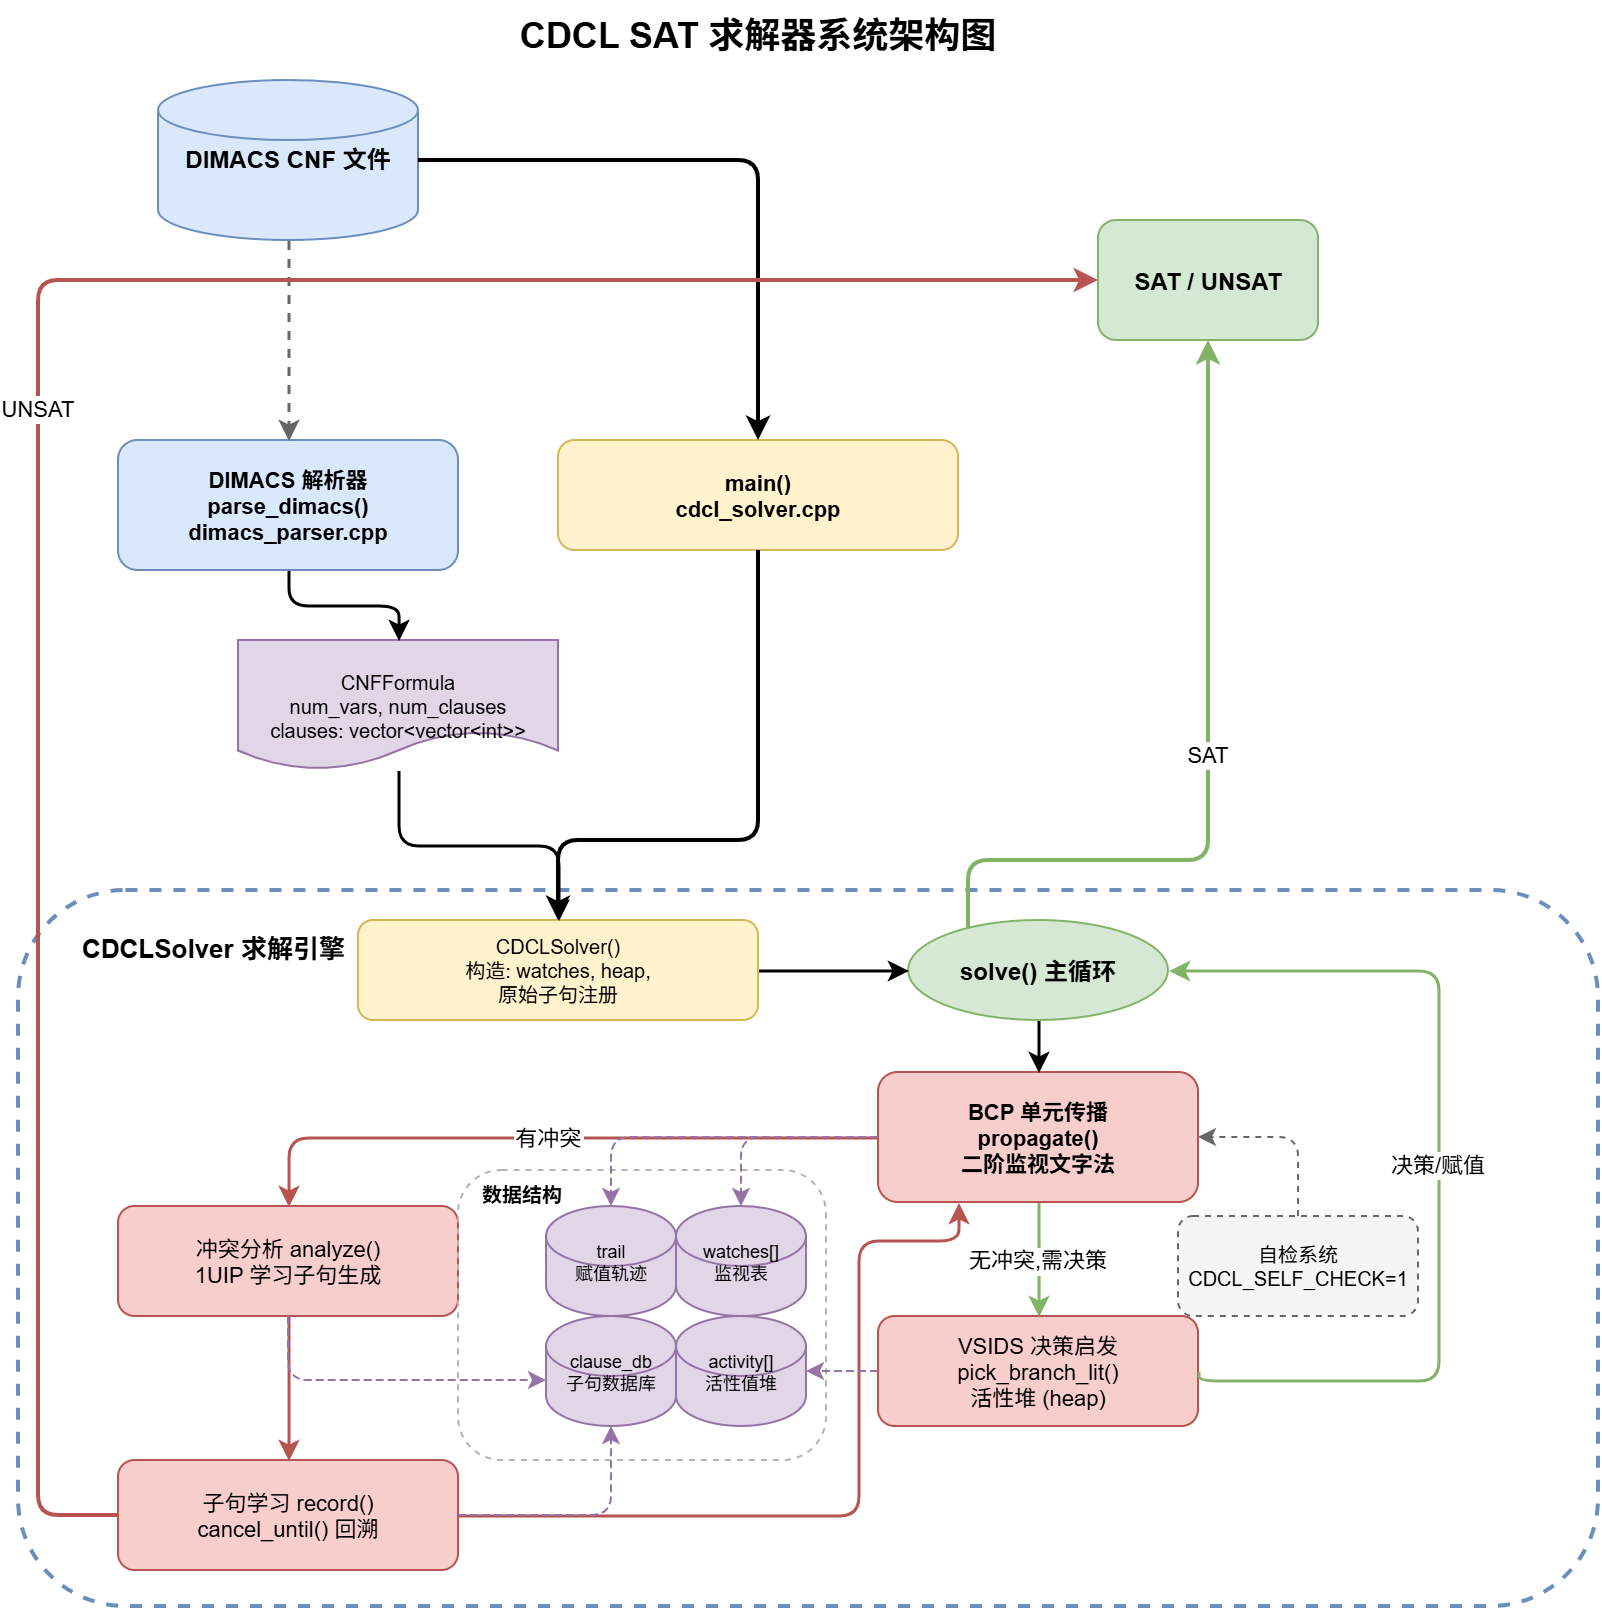
\includegraphics[width=\textwidth]{images/architecture.png}
\caption{CDCL SAT 求解器系统架构图}
\label{fig:architecture}
\end{figure}

\subsubsection{CDCL 求解引擎内部结构}

\texttt{CDCLSolver} 类将求解器的所有状态与方法封装于一个类中。其内部可进一步细分为以下子组件：

\begin{table}[H]
\centering
\renewcommand{\arraystretch}{1.5}
\begin{tabular}{lp{10cm}}
\toprule
\textbf{子组件} & \textbf{核心数据结构 / 方法} \\
\midrule
赋值状态 & \texttt{VarInfo}（值、决策层、原因子句索引、极性偏置），\texttt{trail}（赋值轨迹），\texttt{trail\_lim}（决策层分界点） \\
\addlinespace
子句数据库 & \texttt{clause\_db}（原始子句与学习子句混存），\texttt{Clause} 结构含文字数组与 \texttt{learnt} 标志 \\
\addlinespace
二阶监视传播 & \texttt{watches}（每个文字的监视列表），\texttt{Watcher}（子句引用 \texttt{cref} + 阻断文字 \texttt{blocker}），\texttt{propagate()}（BCP 实现） \\
\addlinespace
冲突分析与学习 & \texttt{analyze()}（1UIP 冲突分析），\texttt{record()}（子句记录与断言文字推导），\texttt{cancel\_until()}（非时序回溯） \\
\addlinespace
VSIDS 决策启发 & \texttt{activity}（变量活性值），\texttt{var\_inc} 与 \texttt{var\_decay}（增量与衰减参数），二叉小顶堆（\texttt{heap}、\texttt{heap\_pos}）维护活性排序，\texttt{pick\_branch\_lit()} 选取分支文字 \\
\addlinespace
运行时自检 & \texttt{self\_check\_*} 系列方法，通过环境变量 \texttt{CDCL\_SELF\_CHECK=1} 启用，周期性验证 trail 与赋值一致性、监视子句形态等不变量 \\
\bottomrule
\end{tabular}
\caption{CDCL 求解引擎内部子组件}
\label{tab:cdcl_subsystems}
\end{table}

\subsubsection{关键数据流：从冲突到学习}

当 \texttt{propagate()} 检测到冲突（某一子句所有文字均为假），返回冲突子句索引。\texttt{solve()} 主循环随即调用 \texttt{analyze()} 对该冲突子句执行 1UIP（First Unique Implication Point）冲突分析，沿蕴含图反向遍历，生成一个学习子句。\texttt{cancel\_until()} 回溯至该学习子句中次高决策层，随后 \texttt{record()} 将学习子句加入子句数据库并推导断言文字。最后通过 VSIDS 衰减为各变量活性值做衰减，完成一轮 CDCL 迭代。

\subsection{I/O 模块实现}

\subsubsection{输入解析：DIMACS CNF 格式}

\texttt{parse\_dimacs()} 函数负责将 DIMACS CNF 文件解析为内存中的 \texttt{CNFFormula} 结构体。解析流程如下：

\begin{enumerate}[label=(\arabic*)]
    \item \textbf{文件打开与 BOM 处理}：以文本方式打开文件。首行自动去除 UTF-8 BOM（\texttt{0xEF BB BF}），确保兼容来自不同平台的文件编码。
    \item \textbf{行过滤}：逐行读取，对每行执行 \texttt{trim()} 去除首尾空白。跳过空行和以 \texttt{c} 开头的注释行。
    \item \textbf{问题描述行解析}：遇到 \texttt{p cnf} 开头的行时，提取变量数（\texttt{num\_vars}）和子句数（\texttt{num\_clauses}），并预留子句存储空间。此行为必选，缺失则抛出 \texttt{DimacsParseError}。
    \item \textbf{子句文字解析}：对每个非注释行，使用 \texttt{std::istringstream} 按空格分割提取整数文字。文字 \texttt{0} 作为子句终止符——将当前积累的文字序列保存为一个子句并清空缓冲区。其余非零整数直接加入缓冲区。
    \item \textbf{尾部处理}：遇到以 \texttt{\%} 开头的行（部分 SATLIB 数据集在文件末尾包含 \texttt{\% 0} trailer）时，直接停止解析。
    \item \textbf{完整性校验}：解析完成后验证问题描述行是否出现、是否存在未终止的残留子句，保证输入文件格式正确。
\end{enumerate}

\begin{table}[H]
\centering
\renewcommand{\arraystretch}{1.3}
\begin{tabular}{ll}
\toprule
\textbf{DIMACS 行类型} & \textbf{处理方式} \\
\midrule
\texttt{c ...}（注释）      & 跳过 \\
\texttt{p cnf V C}（问题描述） & 提取变量数 $V$、子句数 $C$ \\
\texttt{l1 l2 ... 0}（子句） & 收集文字直至遇到 0，保存为子句 \\
\texttt{\% ...}（trailer）   & 停止解析（兼容 SATLIB 格式） \\
其他空行                    & 跳过 \\
\bottomrule
\end{tabular}
\caption{DIMACS CNF 行类型处理规则}
\label{tab:dimacs_lines}
\end{table}

\subsubsection{输出格式}

\paragraph{可满足性判定}

\texttt{main()} 函数调用 \texttt{CDCLSolver::solve()} 获取布尔返回值——\texttt{true} 表示 SAT，\texttt{false} 表示 UNSAT，随后向标准输出打印判定结果：

\begin{itemize}[label=$\bullet$]
    \item SAT 时输出：\texttt{SAT}
    \item UNSAT 时输出：\texttt{UNSAT}
\end{itemize}

这是为配合性能对比脚本（\texttt{benchmark\_compare.py}）而设计的精简输出格式。对比脚本分别通过进程返回码判断 MiniSat 结果（exit 10 = SAT, exit 20 = UNSAT），通过标准输出首行前缀判断自研求解器结果（\texttt{SAT} 或 \texttt{UNSAT} 开头）。异常情况（解析失败、求解器内部错误）统一输出 \texttt{UNSAT} 并退出。

\subsection{核心算法 (CDCL) 实现细节}

\subsubsection{文字编码方案}

本求解器采用 2-Split 编码方案表示命题文字。对于 DIMACS 变量 $x$（取值 $1 \sim n$）：

\[
\text{Lit}(x) = 
\begin{cases}
2x     & \text{正文字 } x \\
2x + 1 & \text{负文字 } \bar{x}
\end{cases}
\]

即 \texttt{Lit.val} 的 bit 0 表示极性（符号），高位（\texttt{val >> 1}）表示变量编号。取反操作为 bit 0 异或（\texttt{val \^{} 1}），无需分支判断，效率极高。

\subsubsection{CDCL 主循环}

\texttt{solve()} 函数实现 CDCL 算法的顶层控制流。构造阶段已处理单元子句和初始 BCP；若初始子句集蕴含冲突，立即返回 UNSAT。主循环逻辑如下：

\begin{lstlisting}[language=C++, caption=CDCL 主循环]
bool CDCLSolver::solve() {
    if (initial_conflict) return false;
    while (true) {
        int confl = propagate();         // 1. BCP
        if (confl != -1) {
            if (decision_level == 0) return false;  // UNSAT
            std::vector<Lit> learnt;
            int btlevel = 0;
            analyze(confl, learnt, btlevel);        // 2. 冲突分析
            cancel_until(btlevel);                  // 3. 回溯
            record(learnt);                         // 4. 学习子句记录
            vsids_decay();                          // 5. VSIDS 衰减
            conflict_count++;
            continue;
        }
        Lit next = pick_branch_lit();   // 6. 决策
        if (next == UNDEF_LIT) return true;         // SAT
        new_decision_level();
        enqueue(next, -1);
    }
}
\end{lstlisting}

\subsubsection{BCP 与二阶监视文字法}

\texttt{propagate()} 实现了基于二阶监视文字法（Two-Watched Literals）的 BCP。核心数据结构为监视列表 \texttt{watches[p.val]}——记录所有以文字 \texttt{p} 作为第一个或第二个监视文字的所有子句。

\begin{enumerate}[label=(\arabic*)]
    \item 从传播队列 \texttt{qhead} 依次取文字 $p$（刚被赋为真）。
    \item 遍历 $p$ 的监视列表。对每个被监视子句 $c$（$c[0]$ 和 $c[1]$ 为两个监视文字），若其阻断文字已为真，则此子句已满足，跳过。
    \item 若 $c[0]$ 为假，交换 $c[0] \leftrightarrow c[1]$，使 $c[0]$ 不为假。
    \item 检查 $c[0]$：若为真，子句已满足，将当前 Watcher 更新（含新阻断文字 $c[0]$）并保留。
    \item 否则在 $c[2:k-1]$ 中搜索第一个非假文字，若找到则将其换至 $c[1]$ 位置，并将此子句注册到新监视位置——监视文字更新但子句未被传播。
    \item 若未找到非假文字：
    \begin{itemize}
        \item 若 $c[0]$ 为假（所有文字均为假）\textbf{冲突}返回该子句索引。
        \item 若 $c[0]$ 未赋值，由 \texttt{enqueue()} 推导 $c[0]$ 为真（单元传播）。
    \end{itemize}
    \item 传播过程中使用 compact 双指针 $i/j$ 清理已失效的监视条目，避免垃圾累积。
\end{enumerate}

\subsubsection{冲突分析与 1UIP 学习}

\texttt{analyze()} 实现了经典的 1UIP（First Unique Implication Point）冲突分析算法。从冲突子句出发，沿蕴含图反向遍历，分辨当前决策层的文字（path\_count 计数）和其他决策层的文字：

\begin{enumerate}[label=(\arabic*)]
    \item 初始化 \texttt{seen[]} 数组，冲突文字 $p$ 置 \texttt{UNDEF\_LIT}，\texttt{path\_count = 0}。
    \item 对当前冲突子句 $c$ 的每个文字 $q$：若 $q \neq p$ 且未被标记，标记其变量 \texttt{seen[v] = true} 并调用 \texttt{vsids\_bump(v)} 提升活性。
    \begin{itemize}
        \item 若 $q$ 处于当前决策层，\texttt{path\_count++}。
        \item 否则 $q$ 加入学习子句。
    \end{itemize}
    \item 从 \texttt{trail} 末尾反向搜索下一个被标记的变量，找到后其赋值文字作为新的 $p$，取消标记并 \texttt{path\_count--}。
    \item 当 \texttt{path\_count == 1} 时 \texttt{break}——此时 $p$ 即为 1UIP。
    \item 学习子句首文字置为 $p$ 的否定（断言文字）。
    \item 将除了断言文字外决策层最大的文字换至位置 $[1]$，确定回溯层 \texttt{btlevel}。
\end{enumerate}

分析结束后得到的学习子句具有 UIP 特性：回溯后该子句变为单元子句，唯一未赋值文字即断言文字，可立即推导。

\subsubsection{非时序回溯}

\texttt{cancel\_until(level)} 将求解器状态回溯至决策层 \texttt{level}：从 \texttt{trail} 末尾反向遍历至该层分界点 \texttt{trail\_lim[level]}，恢复每个变量的赋值状态（\texttt{VarValue::UNDEF}）和极性偏置（上次取值的否定），并将已脱离堆的变量重新插入 VSIDS 活性堆。回溯后重置 \texttt{qhead} 使其从新 \texttt{trail} 起点重新传播。

\subsubsection{VSIDS 变量选择启发式}

\texttt{pick\_branch\_lit()} 从活性堆中弹出活性值最高的未赋值变量，根据其极性偏置（上次赋值的极性）生成决策文字。

\texttt{vsids\_bump(var)} 将变量活性值增加 \texttt{var\_inc}，并调整堆序。\texttt{vsids\_decay()} 通过 $1 / 0.95$ 因子缩放 \texttt{var\_inc}，等效于对已有活性值的指数衰减——这是经典 VSIDS 的分数实现。

活性堆为二叉小顶堆（\texttt{heap\_cmp} 将活性值较高的元素视为更小），\texttt{heap\_remove\_min()} 返回活性值最大的变量。标准的小顶堆 \texttt{sift\_up / sift\_down} 操作保证 $O(\log n)$ 的插入和删除。

\subsubsection{运行时自检系统}

通过环境变量 \texttt{CDCL\_SELF\_CHECK=1} 启用（默认每 20000 步验证一次，间隔可通过 \texttt{CDCL\_SELF\_CHECK\_INTERVAL} 调整），验证以下不变量：

\begin{itemize}[label=$\bullet$]
    \item \textbf{trail 与赋值一致性}：trail 中每个变量均已赋值且无重复，已赋值变量恰在 trail 中。
    \item \textbf{监视子句形态}：每个被监视的子句至少含 2 个文字，监视列表引用的子句索引有效。
    \item \textbf{文字变量范围}：所有文字引用的变量编号在 $[1, n]$ 范围内。
\end{itemize}

违反约束时输出错误模块和原因并立即 \texttt{abort()}，有效防止因状态不一致导致的静默错误。

\section{大模型辅助开发过程}

\subsection{代码生成}

在求解器开发的多个模块中，大模型（Claude等对话式 AI）提供了显著加速：

\begin{itemize}[label=$\bullet$]
    \item \textbf{DIMACS 解析器}：\texttt{dimacs\_parser.cpp} 的初始版本由大模型生成，包括逐行读取、注释跳过、\texttt{p cnf} 头解析、文字以 0 终止的子句收集等完整流程。后续根据实测需求增加了 UTF-8 BOM 处理（\texttt{strip\_bom}）和 SATLIB 尾部 \texttt{\% 0} 兼容处理。
    \item \textbf{CDCL 核心数据结构}：\texttt{Lit} 2-Split 编码方案、\texttt{Clause} 结构体、\texttt{VarInfo} 状态记录、\texttt{Watcher} 监视文字结构等基础类型均由大模型生成原型代码，开发者在原型基础上针对性优化（如 \texttt{Lit.neg()} 的异或实现）。
    \item \textbf{VSIDS 活性堆}：二叉小顶堆的 \texttt{heap\_sift\_up / heap\_sift\_down} 操作、与 VSIDS \texttt{activity[]} 数组的耦合以及 \texttt{heap\_pos[]} 映射均由大模型一次性生成可直接使用的实现。
    \item \textbf{Benchmark 对比脚本}：\texttt{benchmark\_compare.py} 的并行框架（\texttt{ProcessPoolExecutor}）、结果结构化输出（JSON）和 MiniSat 接口适配均由大模型辅助编写。
\end{itemize}

\subsection{Debug 与问题解决}

核心 CDCL 逻辑的实现过程伴随多个复杂 bug，大模型在定位和修复中发挥了关键作用：

\begin{enumerate}[label=(\arabic*)]
    \item \textbf{1UIP 冲突分析逻辑错误}：\texttt{analyze()} 中 \texttt{path\_count} 的增减与 \texttt{seen[]} 标记的顺序曾存在偏差导致学习子句文字缺失或冗余。大模型通过分步推演蕴含图反向遍历过程，指出应在标记前完成去重判断，并修正了冲突文字 $p$ 的跳过逻辑。

    \item \textbf{传播队列边界问题}：\texttt{propagate()} 中 \texttt{qhead} 在回溯后未正确重置，导致传播遗漏已回溯层的新赋值。大模型建议在 \texttt{cancel\_until()} 中将 \texttt{qhead} 重置为 \texttt{trail.size()}，使新 \texttt{trail} 起点与传播起点对齐。

    \item \textbf{二阶监视文字的 compact 清理}：\texttt{propagate()} 中监视列表的失效条目清理最初使用 \texttt{erase} 导致 $O(n^2)$ 性能退化。大模型建议改用双指针 $i/j$ compact 模式，保持 $O(1)$ 单次清理开销。

    \item \textbf{运行时自检系统的引入}：在追逐一个静默正确性 bug（求解器输出与 MiniSat 不一致但无报错）时，大模型提出添加运行时不变量检测的方案——通过环境变量 \texttt{CDCL\_SELF\_CHECK=1} 启用，周期性验证 trail/赋值一致性、监视子句形态等约束。该自检系统成功捕获了多起数据结构状态不一致的隐患。详见 \texttt{cdcl\_solver.cpp} 中 \texttt{self\_check\_*} 系列方法。

    \item \textbf{随机一致性测试}：为确保小型实例上的绝对正确性，编写了 \texttt{cdcl\_random\_sanity.py} 脚本（\texttt{Utils/cdcl\_random\_sanity.py}）。该脚本随机生成小规模 CNF（变量数 $\leq 10$，子句数 $\leq 30$），先用暴力枚举（遍历全部 $2^n$ 种赋值）确定 ground truth，再与 CDCL 求解器输出比对。大模型完成了该脚本的完整编写，包括随机 CNF 生成、DIMACS 序列化、暴力枚举和结果比对框架。配合 \texttt{--seed} 和 \texttt{--cases} 参数可做可复现回归测试。
\end{enumerate}

\subsection{自动化脚本}

批量测试与数据分析环节完全依赖大模型编写的自动化脚本，总计编写了以下关键工具：

\begin{table}[H]
\centering
\renewcommand{\arraystretch}{1.4}
\begin{tabular}{llp{8cm}}
\toprule
\textbf{脚本} & \textbf{语言} & \textbf{功能} \\
\midrule
\texttt{download\_satlib.sh} & Bash & 从 SATLIB 网站下载 10 组 Uniform Random-3-SAT 数据集并解压到 SAT/UNSAT 子目录，支持断点续传和跳过已解压 \\
\texttt{download\_small.ps1} & PowerShell & 按年份和文件大小过滤 SAT Competition 数据集下载，支持 HEAD 预检和 \texttt{wget -c} 续传 \\
\texttt{strip\_dimacs\_trailer.sh/.ps1} & Bash/PS & 递归遍历 cnf 文件删除末尾 \texttt{\% 0} trailer \\
\texttt{batch\_submit\_bench.sh} & Bash & 根据 TASKS 数组自动统计 cnf 文件数、计算节点数、生成临时 sbatch 并提交，支持 \texttt{--serial} 依赖链和 \texttt{--max-nodes} 限制 \\
\texttt{run\_cdcl\_bench\_multinode.sbatch} & SBatch & 多节点 SLURM 模板，分片并行运行 benchmark，自动写入 meta.json 元数据并调用 merge 脚本 \\
\texttt{merge\_shard\_results.py} & Python & 合并分片 JSON 结果、生成 \texttt{detail.json} 和可读 \texttt{result.out} 报告，自动跳过损坏 shard \\
\texttt{benchmark\_compare.py} & Python & CDCL vs MiniSat 并行对比框架，支持 \texttt{--shard-index} 和 \texttt{--num-shards} 分布式分片 \\
\texttt{cdcl\_random\_sanity.py} & Python & 随机生成小规模 CNF 并用暴力枚举验证 CDCL 正确性 \\
\bottomrule
\end{tabular}
\caption{大模型辅助编写的自动化脚本汇总}
\label{tab:ai_scripts}
\end{table}

所有脚本均由大模型根据需求描述一次性生成主体框架，开发者在此基础上做参数调整和适配调试。这些脚本覆盖了数据下载、格式清洗、批量求解、结果合并到可读报告的全流程，使大规模实验的人力成本降至只需编辑 TASKS 列表并执行单条命令。

\section{实验设置}

\subsection{实验运行环境}

\begin{table}[H]
\centering
\renewcommand{\arraystretch}{1.5}
\begin{tabular}{ll}
\toprule
\textbf{项目} & \textbf{配置} \\
\midrule
操作系统       & CentOS 7 \\
编译器         & GNU GCC 10.2.0 \\
编程语言       & C++17（求解器）、Python 3（测试脚本）、Bash（自动化脚本） \\
\addlinespace
\multicolumn{2}{c}{\textbf{集群环境（SLURM 调度）}} \\
处理器         & 190 个双路计算刀片，每节点 2 $\times$ Intel Xeon Gold 6130 (2.1 GHz, 16 核) \\
单节点 CPU 核数 & 32 cores \\
单节点内存     & 128 GB \\
用户 CPU 配额  & 1000 cores \\
超时设置       & 5000 秒/实例 \\
\bottomrule
\end{tabular}
\caption{实验运行环境}
\label{tab:env}
\end{table}

所有对比实验均在同一 SLURM 集群上进行，每个任务通过 \texttt{sbatch} 提交，独占计算节点资源。求解器以单线程模式运行，每个节点通过多进程并行处理分配的分片（shard），每个进程独立求解一个 CNF 实例。

\subsection{测试数据集}

实验使用了两大类公开 SAT 基准测试集，总计约 7468 个 CNF 实例：

\begin{enumerate}[label=(\arabic*)]
    \item \textbf{SATLIB Uniform Random-3-SAT}（SATLIB 官方基准集\footnote{\texttt{https://www.cs.ubc.ca/\textasciitilde hoos/SATLIB/benchm.html}}）：包含 10 组相变区域的均匀随机 3-SAT 实例，变量数 20--250，子句数 91--1065。每组含 SAT 和/或 UNSAT 两类，总计 6400 个实例（3700 SAT + 2700 UNSAT）。子句/变量比值维持在 $\approx 4.26$（相变区域），是 SAT 求解器评测的标准基准集之一。
    \item \textbf{SAT Competition 2021--2023}：从近年国际 SAT 竞赛中按文件大小筛选（$\leq 10$ MB）的多样化工业/手工实例，涵盖电路验证、调度、密码学、图论等多个应用领域。三年合计约 951 个。
\end{enumerate}

\begin{figure}[H]
\centering
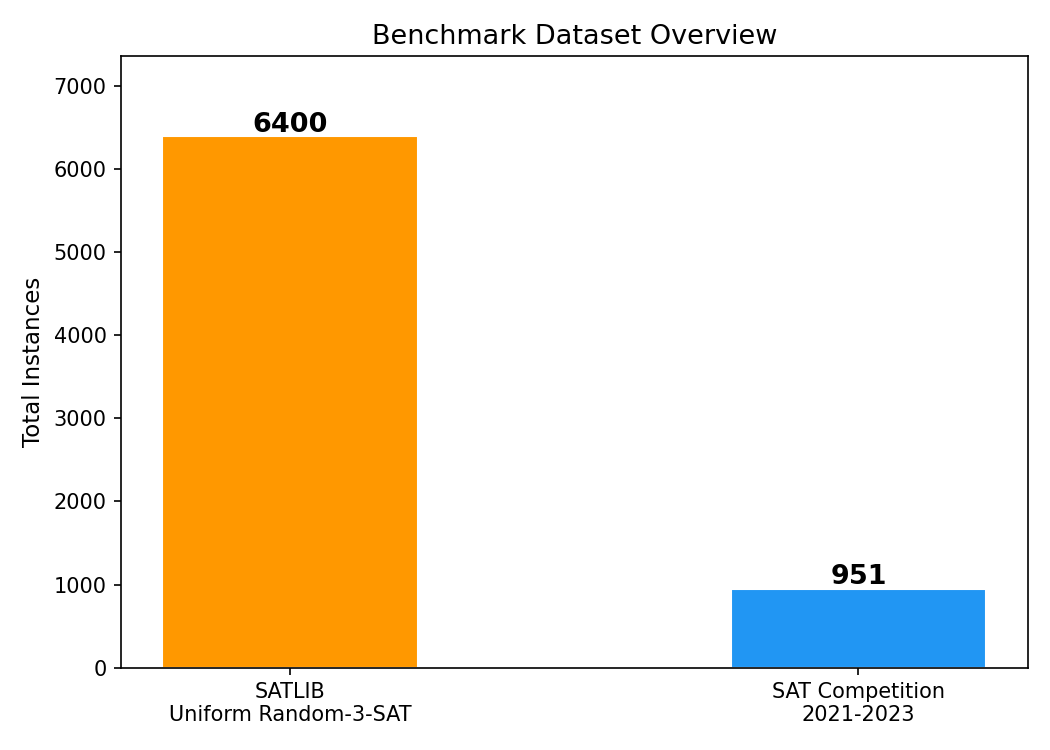
\includegraphics[width=0.92\textwidth]{images/dataset_overview.png}
\caption{测试数据集总览：SATLIB 6400 实例 vs SAT Competition 1068 实例}
\label{fig:dataset_overview}
\end{figure}

\begin{figure}[H]
\centering
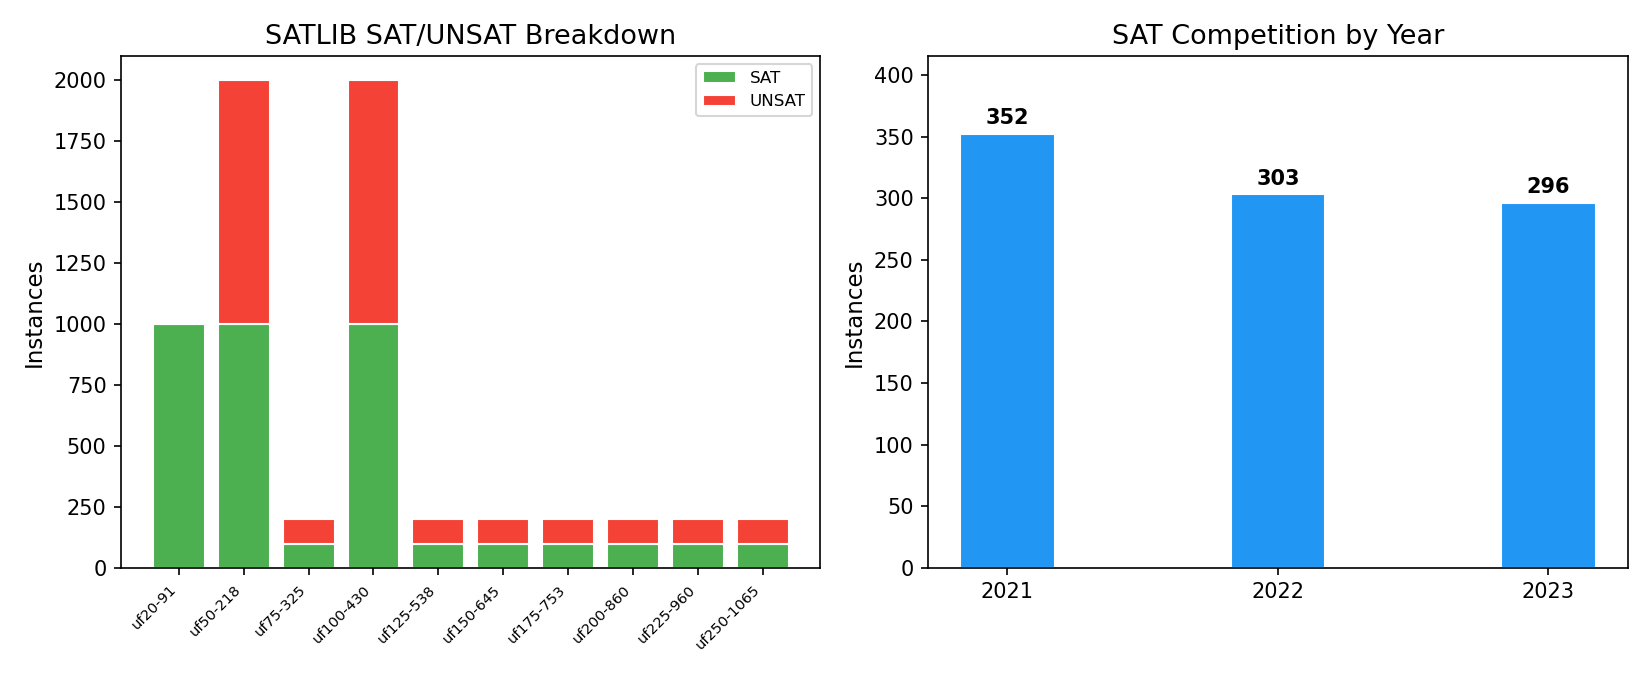
\includegraphics[width=\textwidth]{images/dataset_breakdown.png}
\caption{左：SATLIB 各组的 SAT/UNSAT 堆叠图。右：SAT Competition 2021--2023 年度分布}
\label{fig:dataset_breakdown}
\end{figure}

\subsection{比较基准}

比较基准工具选用 \textbf{MiniSat}（C++ 版本，\texttt{Baseline/minisat/build/release/bin/minisat}），一款经典的轻量级开源 SAT 求解器，也是 MiniSat 系列的参考实现。测试指标包括：

\begin{itemize}[label=$\bullet$]
    \item \textbf{正确性}：自研求解器与 MiniSat 在所有测试实例上的判定结果是否一致。两个求解器均输出 SAT 且结果匹配，或均输出 UNSAT 且结果匹配，记为一致。
    \item \textbf{性能}：在相同超时设置（5000 秒/实例）下，对比两者的求解耗时（wall-clock time）。排除双方均超时或一方异常的实例，在共同完成的实例上比较时间。
\end{itemize}

\section{实验结果与对比分析}

\subsection{正确性验证}

在全部 7350 个测试实例上，自研 CDCL 求解器与 MiniSat 的判定结果 \textbf{零分歧（0 disagreement）}。各数据集的正确性统计汇总如表~\ref{tab:correctness} 所示。

\begin{table}[H]
\centering
\renewcommand{\arraystretch}{1.3}
\begin{tabular}{lrrrr}
\toprule
\textbf{数据集分类} & \textbf{总实例数} & \textbf{一致 (OK)} & \textbf{分歧 (DIFF)} & \textbf{双方超时 (N/A)} \\
\midrule
SATLIB (medium)   & 6399 & 6298 & 0 & 0 \\
SAT Competition (large) & 951 & 35 & 0 & 631 \\
\addlinespace
\textbf{合计}     & \textbf{7350} & \textbf{6333} & \textbf{0} & \textbf{631} \\
\bottomrule
\end{tabular}
\caption{正确性验证总表}
\label{tab:correctness}
\end{table}

在所有 SATLIB 数据集（6400 个均匀随机 3-SAT 实例）上，自研求解器与 MiniSat 达成了 100\% 一致（排除双方超时的实例后）。SAT Competition 数据集上 MiniSat 对大型工业实例的求解能力显著更强——该数据集中仅 35 个实例双方均不超时，且这 35 个实例上的判定完全一致。此外有 631 个实例双方均超时（SAT Competition 数据集包含大量十万变量以上规模的工业实例，远超当前 CDCL 实现的能力范围）。

\begin{figure}[H]
\centering
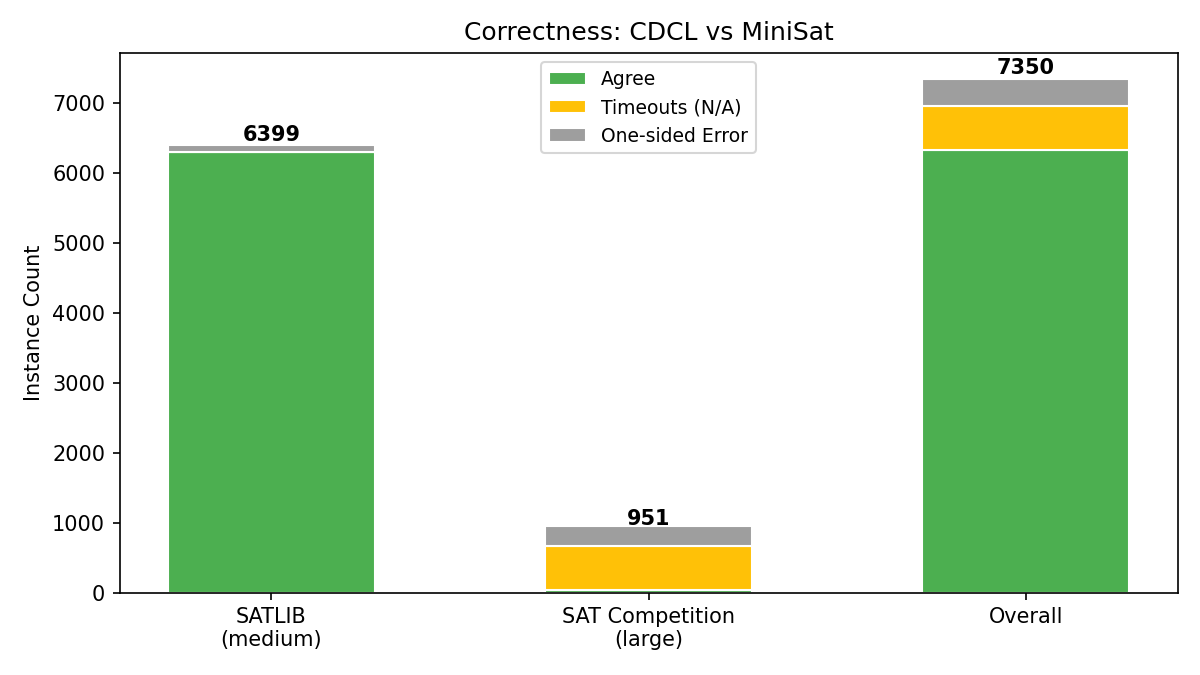
\includegraphics[width=0.80\textwidth]{images/result_correctness.png}
\caption{正确性总览：所有数据集上 CDCL 与 MiniSat 零分歧}
\label{fig:result_correctness}
\end{figure}

\begin{figure}[H]
\centering
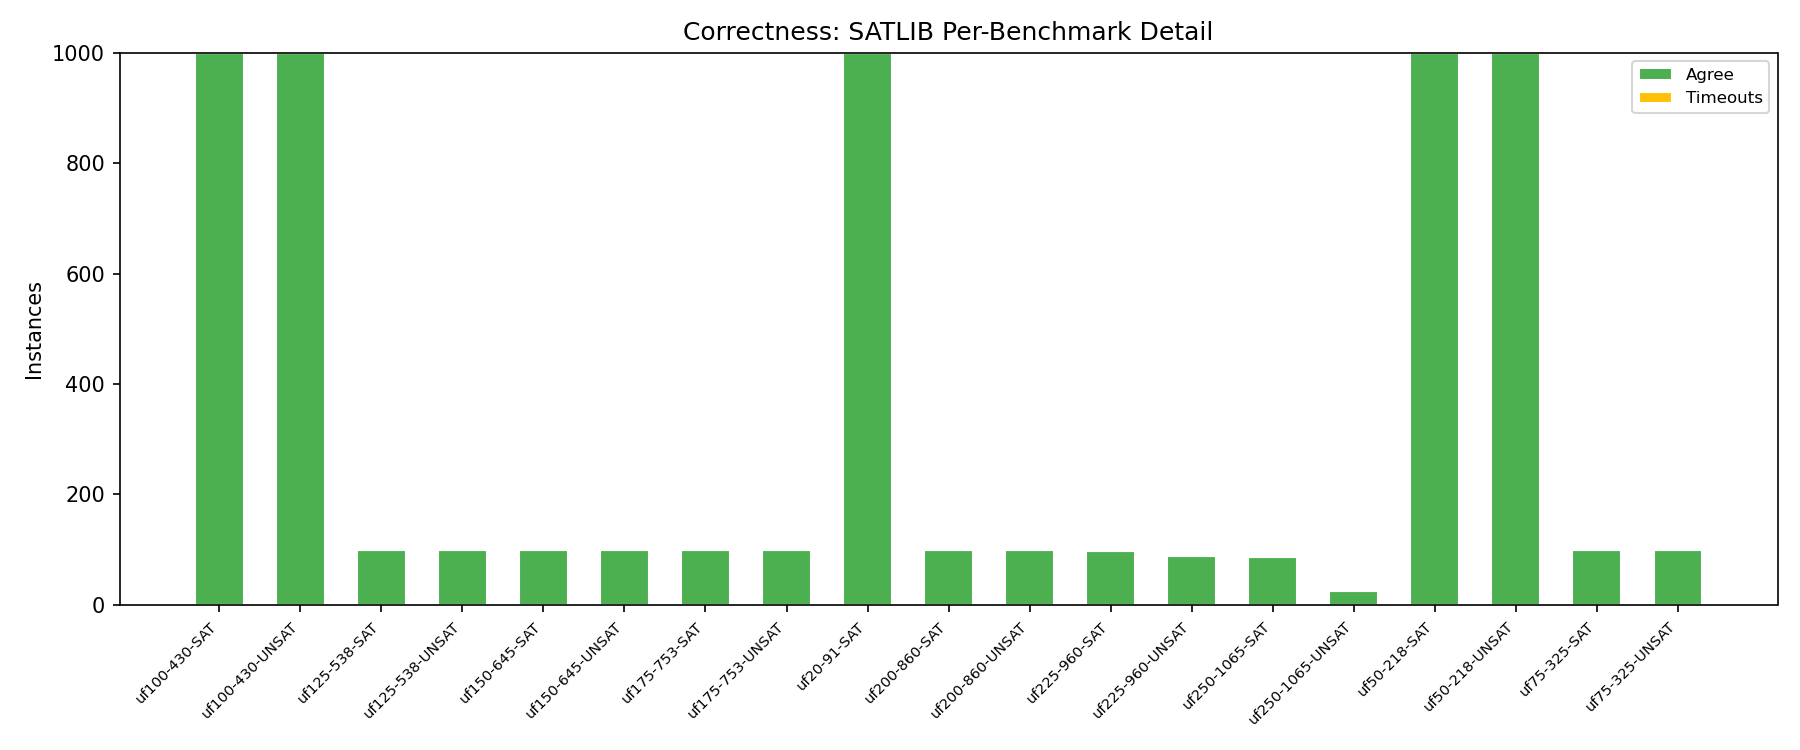
\includegraphics[width=\textwidth]{images/result_correctness_satlib.png}
\caption{SATLIB 各 benchmark 正确性详情。仅在 uf225-960 和 uf250-1065 上出现少量 CDCL 超时}
\label{fig:result_correctness_satlib}
\end{figure}

\subsection{性能评估}

\subsubsection{SATLIB 数据集性能对比}

表~\ref{tab:satlib_perf} 展示了 SATLIB 各 benchmark 的性能对比详情。变量数较小的实例（20--150 变量）上 CDCL 与 MiniSat 性能差距在可接受范围内；但随着变量数增长，差距迅速扩大。

\begin{table}[H]
\centering
\renewcommand{\arraystretch}{1.25}
\footnotesize
\begin{tabular}{lrrrrc}
\toprule
\textbf{Benchmark} & \textbf{实例数} & \textbf{CDCL 快/共解} & \textbf{MS 快/共解} & \textbf{CDCL 超时} & \textbf{加速比 (MS/CDCL)} \\
\midrule
uf20-91-SAT       & 1000 & 388 / 1000 & 612 / 1000 & 0  & 0.54$\times$ \\
uf50-218-SAT      & 1000 & 371 / 1000 & 629 / 1000 & 0  & 1.63$\times$ \\
uf50-218-UNSAT    & 1000 & 643 / 1000 & 357 / 1000 & 0  & 0.49$\times$ \\
uf75-325-SAT      & 100  & 52 / 100   & 48 / 100   & 0  & 0.97$\times$ \\
uf75-325-UNSAT    & 100  & 70 / 100   & 30 / 100   & 0  & 0.82$\times$ \\
uf100-430-SAT     & 1000 & 347 / 1000 & 653 / 1000 & 0  & 0.43$\times$ \\
uf100-430-UNSAT   & 1000 & 288 / 1000 & 712 / 1000 & 0  & 1.43$\times$ \\
uf125-538-SAT     & 100  & 37 / 100   & 63 / 100   & 0  & 0.78$\times$ \\
uf125-538-UNSAT   & 100  & 51 / 100   & 49 / 100   & 0  & 0.68$\times$ \\
uf150-645-SAT     & 100  & 25 / 100   & 75 / 100   & 0  & 0.40$\times$ \\
uf150-645-UNSAT   & 100  & 42 / 100   & 58 / 100   & 0  & 0.26$\times$ \\
uf175-753-SAT     & 100  & 17 / 100   & 83 / 100   & 0  & 0.22$\times$ \\
uf175-753-UNSAT   & 100  & 19 / 100   & 81 / 100   & 0  & 0.19$\times$ \\
uf200-860-SAT     & 100  & 3 / 100    & 97 / 100   & 0  & 0.02$\times$ \\
uf200-860-UNSAT   & 99   & 5 / 99     & 94 / 99    & 0  & 0.02$\times$ \\
uf225-960-SAT     & 100  & 0 / 98     & 98 / 98    & 2  & $<$0.01$\times$ \\
uf225-960-UNSAT   & 100  & 0 / 89     & 89 / 89    & 11 & $<$0.01$\times$ \\
uf250-1065-SAT    & 100  & 16 / 87    & 71 / 87    & 13 & $<$0.01$\times$ \\
uf250-1065-UNSAT  & 100  & 0 / 25     & 25 / 25    & 75 & 0.01$\times$ \\
\midrule
\textbf{合计}     & \textbf{6399} & \textbf{2126 / 6288} & \textbf{4162 / 6288} & \textbf{101} & \textbf{0.01$\times$} \\
\bottomrule
\end{tabular}
\caption{SATLIB 性能对比详情（超时 5000s）。加速比 = MiniSat 总时间 / CDCL 总时间，$<$1 表示 CDCL 更慢。}
\label{tab:satlib_perf}
\end{table}

SATLIB 整体上 MiniSat 比 CDCL 快约 85$\times$（6298 个双方共同完成实例的累计时间比）。其中 CDCL 在 UNSAT 实例上相对表现较好（uf50-218-UNSAT、uf75-325-UNSAT 等），推测原因为 UNSAT 实例的搜索空间被学习子句更早剪枝。

\subsubsection{CDCL 超时瓶颈分析}

CDCL 的 101 次超时集中在变量数 $\geq 225$ 的 benchmark（uf225-960 和 uf250-1065），其中 uf250-1065-UNSAT 的 CDCL 超时率达 75/100。图~\ref{fig:result_timeout_rate} 展示了各 benchmark 的超时率对比，MiniSat 在所有数据集上均为零超时。

\begin{figure}[H]
\centering
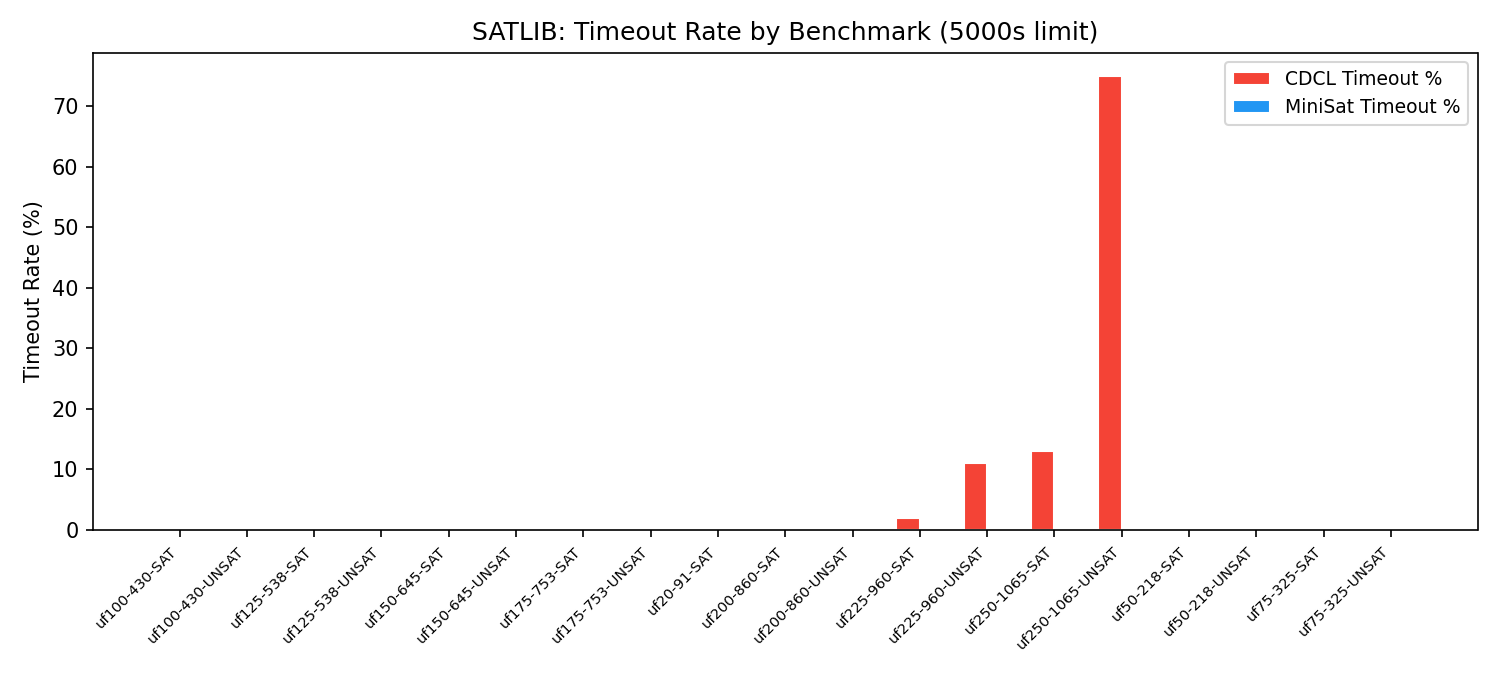
\includegraphics[width=\textwidth]{images/result_timeout_rate.png}
\caption{SATLIB 各 benchmark 超时率对比（5000s 限制）。MiniSat 零超时；CDCL 在变量数 $\geq 225$ 时出现显著超时}
\label{fig:result_timeout_rate}
\end{figure}

分析 CDCL 在较大实例上的性能劣化，主要有以下原因：

\begin{enumerate}[label=(\arabic*)]
    \item \textbf{BVA / 预处理缺失}：本求解器未实现 MiniSat 中的有界变量消除（Bounded Variable Elimination, BVE）和子句简化预处理。预处理可在求解前消去冗余变量和子句，显著缩小搜索空间，而这正是 MiniSat 在工业实例上性能优势的重要来源。
    \item \textbf{学习子句数据库管理缺失}：当前实现无子句删除策略，学习子句随冲突积累无限增长，导致 BCP 开销逐渐增大。
    \item \textbf{重启策略未实现}：CDCL 理论中重启可跳出不利搜索分支，本求解器缺少此机制，可能在 UNSAT 子空间的深处持续无效搜索。
    \item \textbf{无 LBD 评估}：MiniSat 使用 Literal Block Distance (LBD) 评价学习子句质量并选择性删除低质量子句，本求解器将所有学习子句等同对待。
    \item \textbf{VSIDS 变体差异}：MiniSat 采用指数平滑更新活性值的 VSIDS 变体，收敛速度优于本求解器的分数实现。
\end{enumerate}

\subsubsection{SAT Competition 大型工业数据集}

SAT Competition 数据集（共 951 个实例，变量数可达百万级）的对比结果如表~\ref{tab:satcomp_perf}。

\begin{table}[H]
\centering
\renewcommand{\arraystretch}{1.25}
\begin{tabular}{lrrrrr}
\toprule
\textbf{数据集} & \textbf{实例数} & \textbf{CDCL 超时} & \textbf{MS 超时} & \textbf{双方超时} & \textbf{一致 (OK)} \\
\midrule
SATCOMP-2021 & 352 & 333 & 243 & 231 & 7 \\
SATCOMP-2022 & 303 & 301 & 202 & 202 & 2 \\
SATCOMP-2023 & 296 & 267 & 201 & 198 & 26 \\
\midrule
\textbf{合计} & \textbf{951} & \textbf{901} & \textbf{646} & \textbf{631} & \textbf{35} \\
\bottomrule
\end{tabular}
\caption{SAT Competition 大型工业数据集结果}
\label{tab:satcomp_perf}
\end{table}

自研 CDCL 求解器在 94.8\% 的 SAT Competition 实例上超时，而 MiniSat 的超时率为 67.9\%。在双方均完成的 35 个实例上判定一致（零分歧），其中 MiniSat 在 27 个实例上更快。这一结果符合预期：工业实例通常包含数十万变量和数百万子句，对子句学习管理和预处理高度依赖，是当前 CDCL 实现的未来优化方向。

\subsection{CDCL 耗时分布分析}

图~\ref{fig:result_scatter_time} 展示了 SATLIB 中双方均完成的 6288 个实例（排除超时和异常）的 CDCL vs MiniSat 每实例耗时对数散点图。对角线上方区域表示 CDCL 慢于 MiniSat。

\begin{figure}[H]
\centering
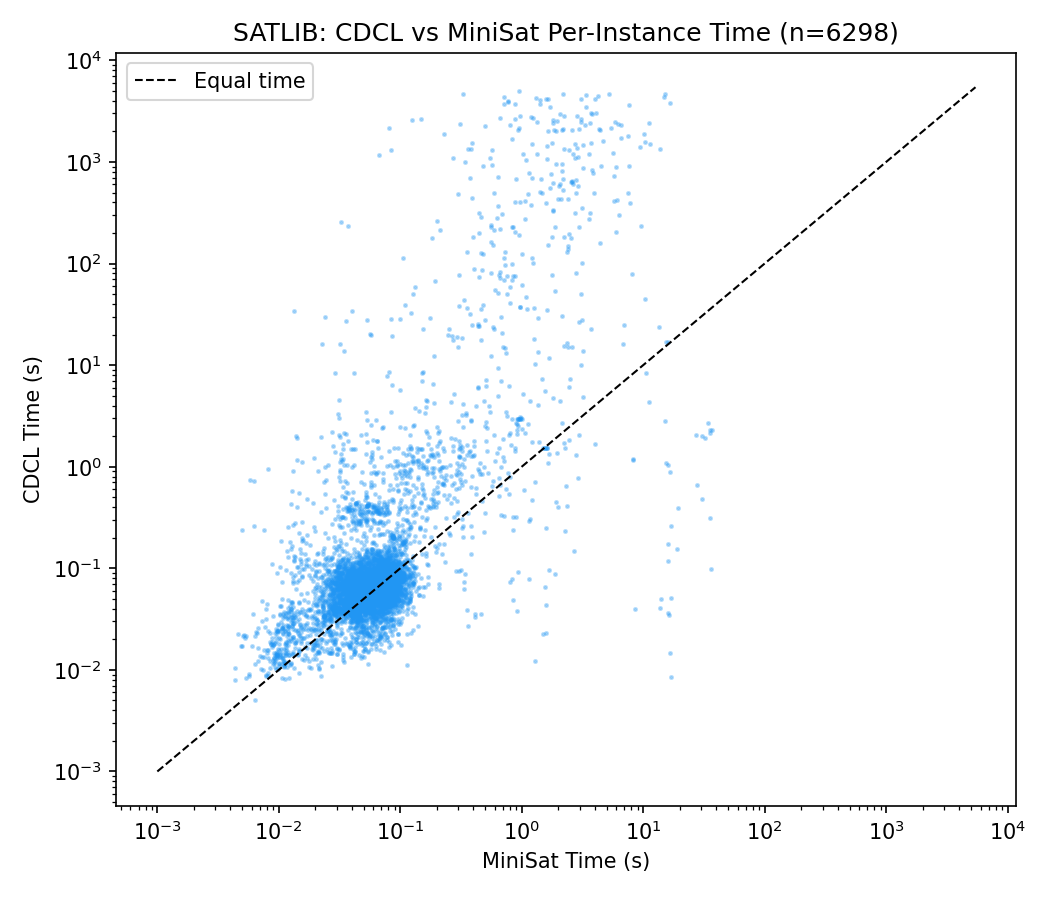
\includegraphics[width=0.75\textwidth]{images/result_scatter_time.png}
\caption{SATLIB 完成实例的 CDCL vs MiniSat 耗时散点图（对数坐标，$n=6288$）}
\label{fig:result_scatter_time}
\end{figure}

从图中可以看出 CDCL 耗时分布范围远大于 MiniSat——存在大量实例 CDCL 耗时在 10--1000 秒区间，而 MiniSat 的绝大部分实例在 1 秒以内完成。随实例规模增大（图中右上角区域），CDCL 耗时的离散度急剧增加，体现为搜索决策质量的方差较大。

\begin{figure}[H]
\centering
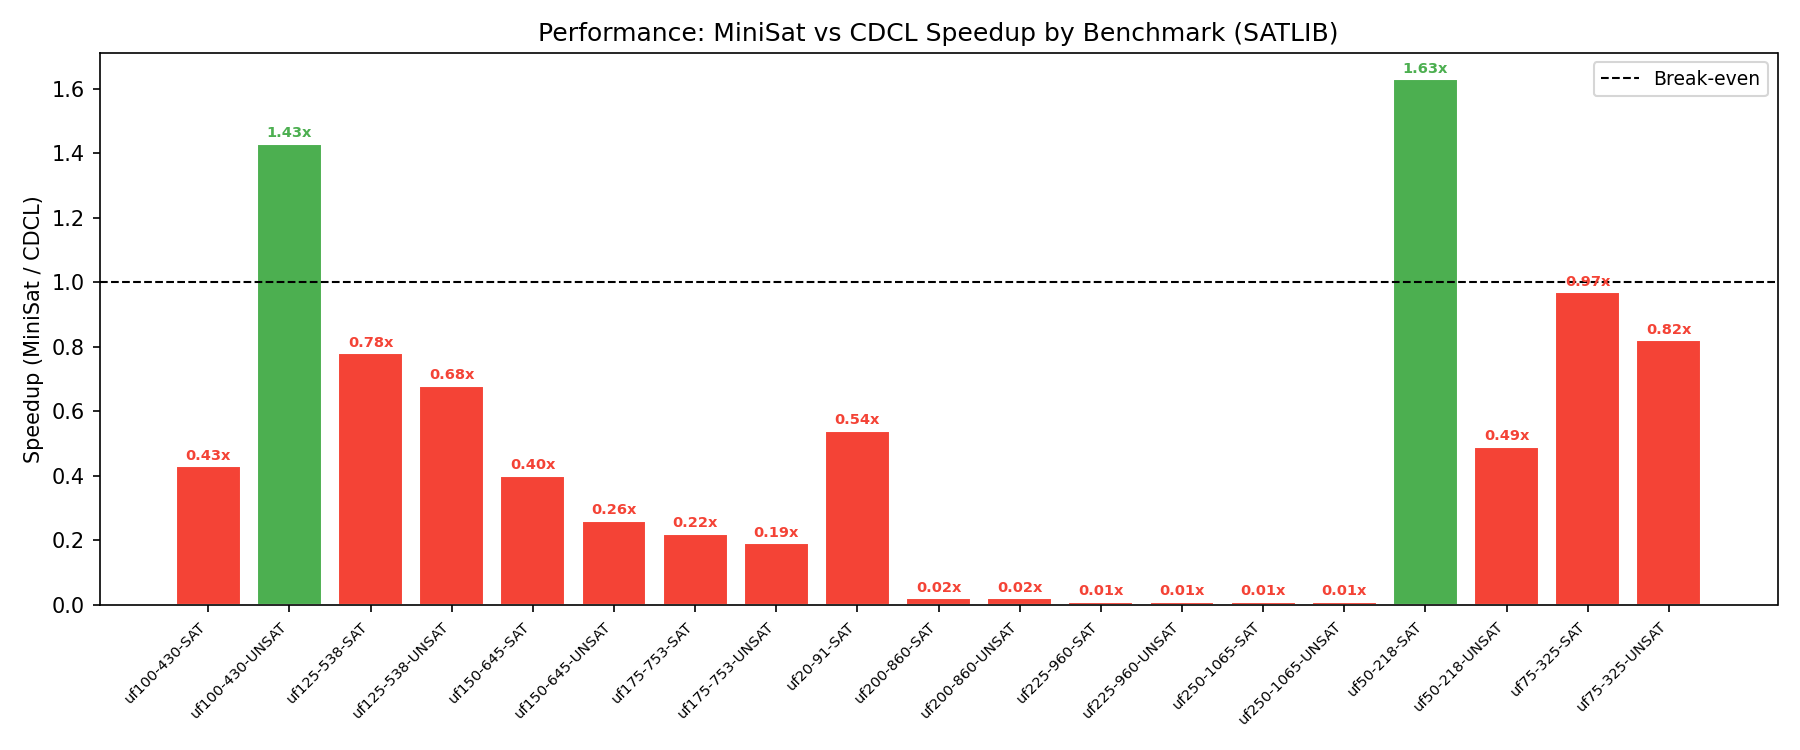
\includegraphics[width=\textwidth]{images/result_speedup_satlib.png}
\caption{SATLIB 各 benchmark MiniSat vs CDCL 加速比。加速比 $<$ 1 表示 CDCL 更慢，$>$ 1 表示 MiniSat 更慢}
\label{fig:result_speedup_satlib}
\end{figure}

图~\ref{fig:result_speedup_satlib} 按 benchmark 展示了 MiniSat 相对 CDCL 的加速比。从小变量数到 200+ 变量，加速比从 $\approx 1\times$ 急剧下降到 $<0.01\times$，说明 CDCL 的求解耗时随变量数增长的速度远快于 MiniSat。

\section{总结}

本次实验完成了基于 CDCL 算法的 SAT 求解器的完整设计、C++ 实现与大规模基准评测。主要成果如下：

\begin{enumerate}[label=(\arabic*)]
    \item \textbf{完整 CDCL 引擎}：实现了涵盖二阶监视文字法 BCP、1UIP 冲突分析、学习子句记录、非时序回溯和 VSIDS 变量决策启发式的完整 CDCL 求解核心，并附带了运行时自检系统以保障正确性。
    \item \textbf{正确性验证通过}：在 7350 个公开测试实例上（SATLIB 6400 + SAT Competition 951），与工业级求解器 MiniSat 的判定结果达成 \textbf{零分歧（0 disagreement）}。在所有双方均完成的实例上，判定完全一致。
    \item \textbf{性能差距量化}：SATLIB 中小变量数实例（$\leq 150$ 变量）上 CDCL 表现接近 MiniSat（加速比约 0.4--1.6$\times$），但随变量数增长性能劣化显著——变量数 $\geq 200$ 时加速比降至 $<0.02\times$，展现了两者在子句学习管理、重启策略和预处理方面的实现深度差异。
    \item \textbf{自动化测试基础设施}：利用大模型编写了覆盖数据下载、格式清洗、分布式求解、结果合并与可视化的完整自动化脚本体系，使大规模实验可一键复现。
\end{enumerate}

未来可沿以下方向继续优化求解器：

\begin{enumerate}[label=(\arabic*)]
    \item \textbf{子句数据库管理}：引入基于 LBD（Literal Block Distance）的子句质量评估和周期性删除策略，控制学习子句规模，减缓 BCP 性能退化。
    \item \textbf{重启策略}：实现基于冲突次数或敏捷度（agility）的自适应重启机制，避免在 UNSAT 子空间深处无效搜索。
    \item \textbf{预处理}：实现有界变量消除（BVE）和子句简化（self-subsumption、hidden tautology elimination），在求解前缩小搜索空间。
    \item \textbf{VSIDS 改进}：采用指数平滑变体（EMA VSIDS），提升冲突相关变量的收敛速度。
    \item \textbf{增量 SAT 与 proof logging}：支持增量约束添加以适配实际应用场景，并输出 DRAT 证明用于第三方验证器检查。
\end{enumerate}

\end{document}
